% !TEX engine = lualatex
\documentclass[aspectratio=169]{fireshonks}

%%%%%%%%%%%%%%%%%%%%%
% PAQUETES
%%%%%%%%%%%%%%%%%%%%%

\setdefaultlanguage{english}
\setotherlanguage[variant=austrian]{german}
\usepackage{tikz}
\usetikzlibrary{arrows.meta, matrix, shapes.geometric, overlay-beamer-styles}
\usepackage[german]{datetime2}
\usepackage{subcaption}
\usepackage{import}
\usepackage{siunitx}
\usepackage{fontawesome5}
\usepackage{emoji}
\sisetup{mode=text, per-mode=symbol}
\captionsetup{font+=scriptsize,justification=centering}
\usepackage{tabularray}
\UseTblrLibrary{booktabs}

%%%%%%%%%%%%%%%%%%%%%
% TEMPLATE
%%%%%%%%%%%%%%%%%%%%%
% Title graphics: BG + logo of the conference
\titlegraphic{
  \begin{tikzpicture}[remember picture, overlay]
    \scoped[on background layer]\node [centered,opacity=0.4] at (current page.center) {
\includegraphics[width=\pagewidth,height=\pageheight,keepaspectratio]{frontmatter/cropped-Try_This_At_Home-1920x1080-1.png}};
    \scoped[on background layer]\node [below left] at (current page.north east) {
\includegraphics[height=4em,keepaspectratio]{frontmatter/annie-shenanigans}};
    % Background: FireShonks  \\
    \scoped[on background layer]\node [above right,align=left,font=\tiny\itshape] at (current page.south west) {
      Seal: \href{https://lethalbit.net}{Aki Van Ness}, CC-BY-SA-4.0
    };
  \end{tikzpicture}
}

%%%%%%%%%%%%%%%%%%
% METADATA
%%%%%%%%%%%%%%%%%%

\title{The Unsung Heroes of Imaging}
\author{amyspark}
\date{\DTMdate{2023-12-27}}

\addbibresource{bibliography.bib}

\begin{document}
\maketitle

\begin{frame}{About me}
  \begin{itemize}[<*>]
    \item Colour spaces, SIMD, build systems... curses are my specialty \emoji{woman-mage}
    \item Currently working with the fine GStreamer folks @ Centricularw
    \item Occasional contributor to a lot of projects
    \item \href{https://www.amyspark.me}{amyspark.me}
  \end{itemize}
\end{frame}
\begin{frame}{Scope}
  \tableofcontents
\end{frame}
\section{Motivation}
\begin{frame}{Motivation}
  \begin{center}
    \Large
    \only<1|handout:0>{\emoji{woman-raising-hand} But wait a minute... what's \emph{YCbCr}?}
    \only<2|handout:0>{\emoji{woman-raising-hand} But wait a minute... what's \emph{a colour space}?}
    \only<3|handout:0>{\emoji{woman-raising-hand} But wait a minute... what's \emph{an ICC profile}?}
    \only<4->{\emoji{woman-raising-hand} But wait a minute... what's \emph{*confusing term here*}?}
  \end{center}
  \uncover<5->{
    \begin{center}That's what we are here for today!\end{center}
  }
\end{frame}
\begin{frame}{Scope}
  \tableofcontents
\end{frame}
\section{Colour management}
\begin{frame}{What is \enquote{colour management}?}
  \begin{definition}
    \enquote{The use of hardware, software, and processes to control and adjust colour among different devices in a (digital) imaging system} \autocite{sharma}
  \end{definition}

  \begin{enumerate}
    \item Why do we need colour management?
    \item How are devices colour managed?
    \item How are colours specified?
  \end{enumerate}
\end{frame}
\begin{frame}{Why do we need colour management?}
  \begin{center}
    \emph{Device-independent colour translation}
  \end{center}

  \begin{itemize}[<+(1)->]
    \item \emoji{thinking} I can haz \colorbox{baseColor3}{\phantom{AKI}} on my screen \textbf{and} in a print?
    \item Each device measures colour in a different way
    \item Formally, given a scene, colour management produces almost identical \autocite{allen}:
          \begin{itemize}
            \item representations from different input devices
            \item representations on different output devices
          \end{itemize}
  \end{itemize}
\end{frame}
\begin{frame}{How are devices colour managed?}
  \enquote{Three Cs} of colour management \autocite{sharma}:
  \begin{itemize}[<+(1)->]
    \item \emph{Calibration}
          \begin{itemize}
            \item set the device up to a known, desired, and \emph{repeatable} state
          \end{itemize}
    \item \emph{Characterization}
          \begin{itemize}
            \item measurement of the response of said device to colour inputs
            \item description in a device-independent manner
            \item this is stored in a \emph{device profile} (and usually embedded in the images it outputs)
          \end{itemize}
    \item \emph{Conversion}
          \begin{itemize}
            \item convert the image between source and destination devices
          \end{itemize}
  \end{itemize}
\end{frame}
\begin{frame}{How are colours specified?}
  Colours are specified as coordinates in a \emph{colour space}.
  \begin{itemize}[<+(1)->]
    \item $n$-dimensional geometrical model
    \item light stimuli (colours) $\leftrightarrow$ vector coordinates
    \item If you've done web dev, you've run across them
          \begin{itemize}
            \item RGB: red-green-blue
            \item HSV: hue-saturation-value
            \item HSL: hue-saturation-lightness
          \end{itemize}
  \end{itemize}
\end{frame}
\begin{frame}{Colour space}
  \begin{itemize}
    \item From a mathematical point of view:
          \begin{itemize}
            \item Coordinate system
            \item A subspace within that system
            \item Each \emph{supported} colour is mapped to a single point inside the subspace
            \item The set of supported colours is the colour space's \emph{gamut}
          \end{itemize}
  \end{itemize}
\end{frame}
\begin{frame}{Colour space}
  \begin{columns}<.->
    \begin{column}<.->{.7\textwidth}
      \begin{itemize}
        \item Construction of a colour space:
              \begin{enumerate}
                \item Three independent, reference stimuli: \emph{primaries}
                      \begin{itemize}
                        \item e.g. in RGB these would be pure red, green, and blue
                      \end{itemize}
                \item White point
                      \begin{itemize}
                        \item the colour of the light source that was used in the scene and/or measurements
                      \end{itemize}
              \end{enumerate}
        \item These colours are represented by their \emph{chromaticity} coordinates
        \item Plotting them in \emph{chromaticity diagrams} reveals the space's gamut
      \end{itemize}
    \end{column}
    \begin{column}<.->{.3\textwidth}
      \begin{figure}
        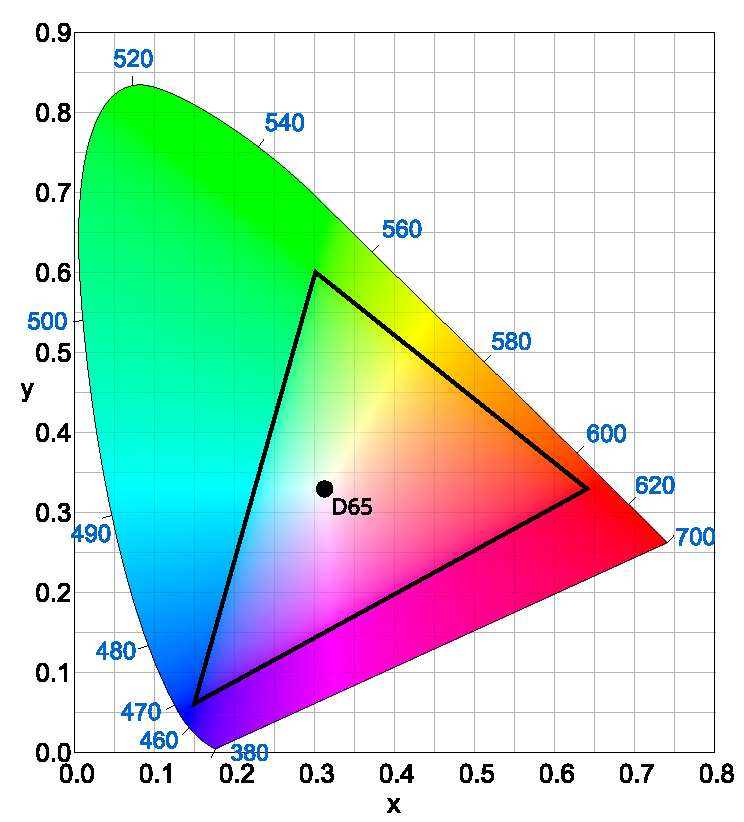
\includegraphics[width=\columnwidth,keepaspectratio]{figures/bt709.pdf}
        \caption*{Source: \href{https://commons.wikimedia.org/wiki/File:CIExy1931.svg}{I, Sakurambo}, \href{http://creativecommons.org/licenses/by-sa/3.0/}{CC BY-SA 3.0}, via Wikimedia Commons}
      \end{figure}
    \end{column}
  \end{columns}
\end{frame}
\begin{frame}{The ICC colour management architecture}
  \begin{itemize}
    \item Modern colour management systems follow the International Colour Consortium's framework \autocite{allen}
    \item \emph{Open-loop} colour management
    \item Calculations are done in a \emph{profile connection space} (PCS)
    \item Intermediate, device-independent colour space
    \item Conversions to/from each device $\equiv$ \emph{transformation} from/to the PCS
          \begin{itemize}
            \item (note the inverted directions)
          \end{itemize}
  \end{itemize}
\end{frame}
\begin{frame}{Open-loop colour management}
  \begin{figure}
    \begin{tikzpicture}[
        node distance=3em and 5em,
        device/.style={align=center, font=\Large},
        pcs/.style={circle, text width=3em, align=center, draw},
        transform/.style={->,shorten >=1pt,>=Latex,semithick}
      ]
      \node (i1) [device] {\emoji{camera}};
      \node (i2) [device, below=of i1] {\emoji{video-camera}};
      \node (i3) [device, below=of i2] {\emoji{movie-camera}};
      \node (pcs) [pcs, right=of i2] {PCS};
      \node (d1) [device, above=of pcs] {\emoji{desktop-computer}};
      \node (d2) [device, below=of pcs] {\emoji{mobile-phone}};
      \node (o1) [device, above right=of pcs] {\emoji{printer}};
      \node (o2) [device, below right=of pcs] {\emoji{printer}};

      \draw[transform] (i1) -- (pcs) node [midway, visible on=<2->] {\emoji{arrows-counterclockwise}};
      \draw[transform] (i2) -- (pcs) node [midway, visible on=<2->] {\emoji{arrows-counterclockwise}};
      \draw[transform] (i3) -- (pcs) node [midway, visible on=<2->] {\emoji{arrows-counterclockwise}};
      \draw[transform] (i1) -- (pcs) node [midway, visible on=<2->] {\emoji{arrows-counterclockwise}};
      \draw[transform] (pcs) -- (d1) node [midway, visible on=<2->] {\emoji{arrows-counterclockwise}};
      \draw[transform] (pcs) -- (d2) node [midway, visible on=<2->] {\emoji{arrows-counterclockwise}};
      \draw[transform] (pcs) -- (o1) node [midway, visible on=<2->] {\emoji{arrows-counterclockwise}};
      \draw[transform] (pcs) -- (o2) node [midway, visible on=<2->] {\emoji{arrows-counterclockwise}};
    \end{tikzpicture}

    \caption*{Adapted from \textcite[viii]{icc}}
  \end{figure}
\end{frame}
\begin{frame}{The ICC colour management architecture}
  Four key components:
  \begin{enumerate}[<+(1)->]
    \item The PCS
    \item The \emph{colour management module}
          \begin{itemize}
            \item A software library that performs all the colour conversions
            \item Usually embedded on your OS, there are also vendor offerings available
          \end{itemize}
    \item The device profiles
          \begin{itemize}
            \item Contain the data to transform between PCS and the device's colour space
            \item \emoji{woman-mage} We'll try to make one of these!
          \end{itemize}
    \item Rendering \emph{intents}
          \begin{itemize}
            \item Exact matches between spaces may not be possible: \emph{out-of-gamut} colours
            \item The CMS needs to \emph{predictably} account for this
          \end{itemize}
  \end{enumerate}
\end{frame}
\begin{frame}{Processing the colour values}
  ICC profiles can process colours in two ways, according to the latest spec (v4.3, \cite*{icc}).
  \begin{itemize}[<+(1)->]
    \item Matrix + TRC
    \item Color look-up tables
  \end{itemize}
\end{frame}
\begin{frame}{Matrix/TRC}
  \begin{itemize}
    \item Combines a $3\times3$ matrix and \emph{tone reproduction curves}
          (gamma/OETF)
    \item Can convert only RGB or greyscale
    \item \textbf{Not stored directly}
    \item One TRC for each channel
    \item Coordinates of the 3 primaries $\rightarrow$ 3x3 matrix
  \end{itemize}
\end{frame}
\begin{frame}{Matrix/TRC}
  This is the flow of a device colour space to PCS conversion:
  \begin{figure}
    \begin{tikzpicture}[
        stage/.style={column sep=0pt, inner xsep=0pt, anchor=center, left delimiter=\lbrack, right delimiter=\rbrack},
        trc/.style={row sep=5pt, column sep=0pt, nodes={font=\LARGE, anchor=center, draw}},
        stage label/.style={inner sep=0pt, anchor=mid},
        transform/.style={->,shorten >=1pt,>=Latex,semithick},
        clut/.style={regular polygon, regular polygon sides=4, inner sep=-0.5em, anchor=center, draw}
      ]
      \matrix [stage, matrix anchor=a2.center] (A) {
        \node (a1) {Channel 1}; \\
        \node (a2) {Channel 2}; \\
        \node (a3) {Channel 3}; \\
      };
      \node [stage label, above=4em of A.center] (l1) {Device space};
      \node [right=1mm of a1.east] (c1) {};
      \node [right=1mm of a2.east] (c2) {};
      \node [right=1mm of a3.east] (c3) {};

      \matrix [trc, right=5em of A.east, matrix anchor=trc2.west] (trc) {
        \node (trc1) {\faChartLine}; \\
        \node (trc2) {\faChartLine}; \\
        \node (trc3) {\faChartLine}; \\
      };

      \node [clut, right=7em of trc, anchor=west] (M) {$\text{Matrix}_{3 \times 3}$};

      \matrix [stage, right=5em of M, matrix anchor=b2.center] (b) {
        \node (b1) {X}; \\
        \node (b2) {Y}; \\
        \node (b3) {Z}; \\
      };
      \node [left=1mm of b1.west] (x) {};
      \node [left=1mm of b2.west] (y) {};
      \node [left=1mm of b3.west] (z) {};

      \path (l1.east) -| (trc.center) node [midway] (l2x) {};
      \node [stage label] at (l2x) {\enquote{B} curves};

      \path (l1.east) -| (b.center) node [midway] (l3x) {};
      \node [stage label] at (l3x) {PCS};

      \draw [transform] (c1) -- ++(2em,0em) |- (trc1.west);
      \draw [transform] (c2) -- ++(2em,0em) |- (trc2.west);
      \draw [transform] (c3) -- ++(2em,0em) |- (trc3.west);

      \path (M.west) |- (x) node [midway] (m1) {};
      \path (M.west) |- (y) node [midway] (m2) {};
      \path (M.west) |- (z) node [midway] (m3) {};

      \draw [transform] (trc1.east) node[above right] {TRC$_{1}$} -- ++(3.5em,0em) |- (m1);
      \draw [transform] (trc2.east) node[above right] {TRC$_{2}$} -- ++(3.5em,0em) |- (m2);
      \draw [transform] (trc3.east) node [above right] {TRC$_{3}$} -- ++(3.5em,0em) |- (m3) ;

      \path (M.east) |- (x) node [midway] (m4){};
      \path (M.east) |- (y) node [midway] (m5){};
      \path (M.east) |- (z) node [midway] (m6){};

      \draw [transform] (m4) -- ++(1.5em,0em) |- (x);
      \draw [transform] (m5) -- ++(1.5em,0em) |- (y);
      \draw [transform] (m6) -- ++(1.5em,0em) |- (z);
    \end{tikzpicture}
    \caption*{Adapted from \textcite[xi]{icc}}
  \end{figure}
\end{frame}
\begin{frame}{Matrix/TRC}
  To go from the PCS to the device colour space, the matrix and curves are inverted.

  The calculations are done by the CMM, no extra effort is needed.

  \begin{figure}
    \begin{tikzpicture}[
        stage/.style={column sep=0pt, inner xsep=0pt, anchor=center, left delimiter=\lbrack, right delimiter=\rbrack},
        trc/.style={row sep=5pt, column sep=0pt, nodes={font=\LARGE, anchor=center, draw}},
        stage label/.style={inner sep=0pt, anchor=mid},
        transform/.style={->,shorten >=1pt,>=Latex,semithick},
        clut/.style={regular polygon, regular polygon sides=4, inner sep=-0.5em, anchor=center, draw}
      ]
      \matrix [stage, matrix anchor=b2.center] (b) {
        \node (b1) {X}; \\
        \node (b2) {Y}; \\
        \node (b3) {Z}; \\
      };
      \node [right=1mm of b1.east] (x) {};
      \node [right=1mm of b2.east] (y) {};
      \node [right=1mm of b3.east] (z) {};

      \node [clut, right=5em of b] (M) {Matrix$_{3 \times 3}^{-1}$};

      \matrix [trc, right=5em of M.east, matrix anchor=trc2.west] (trc) {
        \node (trc1) {\faChartLine}; \\
        \node (trc2) {\faChartLine}; \\
        \node (trc3) {\faChartLine}; \\
      };

      \matrix [stage, matrix anchor=a2.west, right=7em of trc] (A) {
        \node (a1) {Channel 1}; \\
        \node (a2) {Channel 2}; \\
        \node (a3) {Channel 3}; \\
      };
      \node [stage label, above=4em of A.center] (l1) {Device space};
      \node [left=1mm of a1.west] (c1) {};
      \node [left=1mm of a2.west] (c2) {};
      \node [left=1mm of a3.west] (c3) {};

      \path (l1.west) -| (trc.center) node [midway] (l2x) {};
      \node [stage label] at (l2x) {\enquote{B} curves};

      \path (l1.west) -| (b.center) node [midway] (l3x) {};
      \node [stage label] at (l3x) {PCS};

      \draw [transform] (trc1.east)  node[above right] {TRC$_{1}^{-1}$} -- ++(3.5em,0em) |- (c1);
      \draw [transform] (trc2.east) node[above right] {TRC$_{2}^{-1}$} -- ++(3.5em,0em) |- (c2);
      \draw [transform] (trc3.east) node [above right] {TRC$_{3}^{-1}$} -- ++(3.5em,0em) |- (c3);

      \path (M.east) |- (x) node [midway] (m1) {};
      \path (M.east) |- (y) node [midway] (m2) {};
      \path (M.east) |- (z) node [midway] (m3) {};

      \draw [transform] (m1) -- ++(3em,0em) |- (trc1.west);
      \draw [transform] (m2) -- ++(3em,0em) |- (trc2.west);
      \draw [transform] (m3) -- ++(3em,0em) |- (trc3.west) ;

      \path (M.west) |- (x) node [midway] (m4){};
      \path (M.west) |- (y) node [midway] (m5){};
      \path (M.west) |- (z) node [midway] (m6){};

      \draw [transform] (x) -- ++(1.5em,0em) |- (m4);
      \draw [transform] (y) -- ++(1.5em,0em) |- (m5);
      \draw [transform] (z) -- ++(1.5em,0em) |- (m6);
    \end{tikzpicture}
    \caption*{Adapted from \textcite[x]{icc}}
  \end{figure}
\end{frame}
\begin{frame}{n-component color look-up tables}
  \begin{itemize}
    \item $n$-channel colour spaces e.g. CMYK
    \item Alternatively, more complex colour conversions
    \item Each transform direction is \emph{explicitly} stored in separate \emph{tags}
    \item The standard version (required): 8 or 16-bit unsigned integer depth
          \begin{itemize}
            \item \emph{AtoB0} (to PCS) and \emph{BtoA0} (from PCS) tags
          \end{itemize}
    \item Alternative: floating-point depth
          \begin{itemize}
            \item \emph{DtoB0} (to PCS) and \emph{BtoD0} (from PCS) tags
            \item Overrides the former if specified (and the CMM supports it)
          \end{itemize}
  \end{itemize}
\end{frame}
\begin{frame}{n-component color look-up tables}
  \begin{itemize}
    \item \emph{AtoB0} and \emph{BtoA0} are \emph{colour transform} structures
    \item Up to 5 elements, 4 possible ways to use them
    \item Device $\rightarrow$ PCS:
          \begin{enumerate}
            \item B
            \item M-Matrix-B (explicit matrix/TRC)
            \item A-CLUT-B
            \item A-CLUT-M-Matrix-B (the most expressive, also the heaviest storage-wise)
          \end{enumerate}
    \item PCS $\rightarrow$ device: reverse the direction
    \item Note: Matrix has a fourth \emph{offset} column (unlike matrix/TRC)
  \end{itemize}
\end{frame}
\begin{frame}{n-component color look-up tables}
  Device $\rightarrow$ PCS transform:

  \begin{figure}
    \footnotesize
    \begin{tikzpicture}[
        stage/.style={inner xsep=0pt, column sep=5pt, anchor=center, left delimiter=\lbrack, right delimiter=\rbrack, matrix anchor=west},
        trc/.style={row sep=5pt, column sep=0pt, matrix anchor=west, nodes={font=\large, anchor=center, align=center, minimum width=2em}},
        stage label/.style={inner sep=0pt, anchor=mid},
        transform/.style={->,shorten >=1pt,>=Latex,semithick},
        clut/.style={regular polygon, regular polygon sides=4, anchor=west, minimum size=9em, inner sep=0pt, draw}
      ]
      \matrix [stage] (S) {
        \node (s1) {Channel 1};    \\
        \node (s2) {Channel 2};    \\
        \node (s3) {\faEllipsisV}; \\
        \node (sn) {Channel n};    \\
      };
      \node [stage label, above=5em of S.center] (l1) {Device space};
      \node [right=.05em of s1.east] (c1) {};
      \node [right=.05em of s2.east] (c2) {};
      \path (c2) |- (s3) node [midway] (c3) {};
      \node [right=.05em of sn.east] (cn) {};

      \matrix [trc, right=2.5em of S.east] (A) {
        \node [draw] (a1) {\faChartLine}; \\
        \node [draw] (a2) {\faChartLine}; \\
        \node (a3) {\faEllipsisV};        \\
        \node [draw] (an) {\faChartLine}; \\
      };

      \node [clut, right=2em of A.east] (CLUT) { CLUT };

      \matrix [trc, right=2em of CLUT.east] (M) {
        \node [draw] (M1) {\faChartLine}; \\
        \node [draw] (M2) {\faChartLine}; \\
        \node [draw] (M3) {\faChartLine}; \\
      };

      \node [clut, right=2em of M.east] (Matrix) {$\text{Matrix}_{3 \times 4}$};

      \matrix [trc, right=2em of Matrix.east] (B) {
        \node [draw] (b1) {\faChartLine}; \\
        \node [draw] (b2) {\faChartLine}; \\
        \node [draw] (b3) {\faChartLine}; \\
      };

      \matrix [stage, right=2.5em of B.east, ampersand replacement=\&] (PCS) {
        \node (pcs1) {X}; \& \& \node (pcs4) {$\text{L}*$};             \\
        \node (pcs2) {Y}; \& \node {or}; \& \node (pcs5) {$\text{a}*$}; \\
        \node (pcs3) {Z}; \& \& \node (pcs6) {$\text{b}*$};             \\
      };
      \node [left=.05em of pcs1.west] (x) {};
      \node [left=.05em of pcs2.west] (y) {};
      \node [left=.05em of pcs3.west] (z) {};

      \path (l1.east) -| (A.center) node [midway] (l2x) {};
      \node [stage label] at (l2x) {\enquote{A} curves};

      \path (l1.east) -| (CLUT.center) node [midway] (l3x) {};
      \node [stage label, align=center] at (l3x) {Multi-dimensional \\ look-up table};

      \path (l1.east) -| (M.center) node [midway] (l4x) {};
      \node [stage label] at (l4x) {\enquote{M} curves};

      \path (l1.east) -| (B.center) node [midway] (l5x) {};
      \node [stage label] at (l5x) {\enquote{B} curves};

      \path (l1.east) -| (PCS.center) node [midway] (l6x) {};
      \node [stage label] at (l6x) {PCS};

      \draw [transform] (c1.east) -- ++(1em,0em) |- (a1.west);
      \draw [transform] (c2.east) -- ++(1em,0em) |- (a2.west);
      \draw [transform] (c3.east) -- ++(1em,0em) |- (a3.west);
      \draw [transform] (cn.east) -- ++(1em,0em) |- (an.west);

      \path (CLUT.west) |- (s1.east) node [midway] (m1) {};
      \path (CLUT.west) |- (s2.east) node [midway] (m2) {};
      \path (CLUT.west) |- (s3.east) node [midway] (m3) {};
      \path (CLUT.west) |- (sn.east) node [midway] (m4) {};

      \draw [transform] (a1.east) -- ++(1em,0em) |- (m1.center);
      \draw [transform] (a2.east) -- ++(1em,0em) |- (m2.center);
      \draw [transform] (a3.east) -- ++(1em,0em) |- (m3.center);
      \draw [transform] (an.east) -- ++(1em,0em) |- (m4.center) ;

      \path (CLUT.east) |- (x) node [midway] (m5) {};
      \path (CLUT.east) |- (y) node [midway] (m6) {};
      \path (CLUT.east) |- (z) node [midway] (m7) {};

      \draw [transform] (m5.center) -- ++(1em,0em) |- (M1.west);
      \draw [transform] (m6.center) -- (M2.west);
      \draw [transform] (m7.center) -- ++(1em,0em) |- (M3.west);

      \path (Matrix.west) |- (x) node [midway] (Matrix1) {};
      \path (Matrix.west) |- (z) node [midway] (Matrix3) {};

      \draw [transform] (M1.east) -- ++(1em,0em) |- (Matrix1.center);
      \draw [transform] (M2.east) -- (Matrix.west);
      \draw [transform] (M3.east) -- ++(1em,0em) |- (Matrix3.center);

      \path (Matrix.east) |- (x) node [midway] (Matrix4) {};
      \path (Matrix.east) |- (y) node [midway] (Matrix5) {};
      \path (Matrix.east) |- (z) node [midway] (Matrix6) {};

      \draw [transform] (Matrix4.center) -- ++(1em,0em) |- (b1.west);
      \draw [transform] (Matrix5.center) -- (b2.west);
      \draw [transform] (Matrix6.center) -- ++(1em,0em) |- (b3.west);

      \draw [transform] (b1.east) -- ++(1em,0em) |- (x.center);
      \draw [transform] (b2.east) -- (y.center);
      \draw [transform] (b3.east) -- ++(1em,0em) |- (z.center);
    \end{tikzpicture}

    \caption*{Source: \textcite[xii]{icc}}
  \end{figure}
\end{frame}
\begin{frame}{n-component color look-up tables}
  PCS $\rightarrow$ device transform:

  \begin{figure}
    \footnotesize
    \begin{tikzpicture}[
        stage/.style={inner xsep=0pt, column sep=5pt, left delimiter=\lbrack, right delimiter=\rbrack, matrix anchor=west, nodes={anchor=center, align=center}},
        trc/.style={row sep=5pt, column sep=0pt, matrix anchor=west, nodes={font=\large, anchor=center, align=center, minimum width=2em}},
        stage label/.style={inner sep=0pt, anchor=mid},
        transform/.style={->,shorten >=1pt,>=Latex,semithick},
        clut/.style={regular polygon, regular polygon sides=4, anchor=west, minimum size=9em, inner sep=0pt, draw}
      ]
      \matrix [stage, ampersand replacement=\&] (PCS) {
        \node (pcs1) {X}; \& \& \node (pcs4) {$\text{L}*$};             \\
        \node (pcs2) {Y}; \& \node {or}; \& \node (pcs5) {$\text{a}*$}; \\
        \node (pcs3) {Z}; \& \& \node (pcs6) {$\text{b}*$};             \\
      };
      \node [right=.05em of PCS.east] (y) {};
      \path (y) |- (pcs4) node [midway] (x) {};
      \path (y) |- (pcs6) node [midway] (z) {};

      \matrix [trc, right=2.5em of PCS.east] (B) {
        \node [draw] (b1) {\faChartLine}; \\
        \node [draw] (b2) {\faChartLine}; \\
        \node [draw] (b3) {\faChartLine}; \\
      };

      \node [clut, right=2em of B.east] (Matrix) {$\text{Matrix}_{3 \times 4}$};

      \matrix [trc, right=2em of Matrix.east] (M) {
        \node [draw] (M1) {\faChartLine}; \\
        \node [draw] (M2) {\faChartLine}; \\
        \node [draw] (M3) {\faChartLine}; \\
      };

      \node [clut, right=2em of M.east] (CLUT) { CLUT };

      \matrix [trc, right=2em of CLUT.east] (A) {
        \node [draw] (a1) {\faChartLine}; \\
        \node [draw] (a2) {\faChartLine}; \\
        \node (a3) {\faEllipsisV};        \\
        \node [draw] (an) {\faChartLine}; \\
      };

      \matrix [stage, right=2.5em of A.east] (S) {
        \node (s1) {Channel 1};    \\
        \node (s2) {Channel 2};    \\
        \node (s3) {\faEllipsisV}; \\
        \node (sn) {Channel n};    \\
      };
      \node [stage label, above=5em of S.center] (l1) {Device space};
      \node [left=.05em of s1.west] (c1) {};
      \path (c1) |- (s2) node [midway] (c2) {};
      \path (c2) |- (s3) node [midway] (c3) {};
      \path (c3) |- (sn) node [midway] (cn) {};

      \path (l1.east) -| (A.center) node [midway] (l2x) {};
      \node [stage label] at (l2x) {\enquote{A} curves};

      \path (l1.east) -| (CLUT.center) node [midway] (l3x) {};
      \node [stage label, align=center] at (l3x) {Multi-dimensional \\ look-up table};

      \path (l1.east) -| (M.center) node [midway] (l4x) {};
      \node [stage label] at (l4x) {\enquote{M} curves};

      \path (l1.east) -| (B.center) node [midway] (l5x) {};
      \node [stage label] at (l5x) {\enquote{B} curves};

      \path (l1.east) -| (PCS.center) node [midway] (l6x) {};
      \node [stage label] at (l6x) {PCS};

      \draw [transform] (a1.east) -- ++(1em,0em) |- (c1.west);
      \draw [transform] (a2.east) -- ++(1em,0em) |- (c2.west);
      \draw [transform] (a3.east) -- ++(1em,0em) |- (c3.west);
      \draw [transform] (an.east) -- ++(1em,0em) |- (cn.west);

      \path (CLUT.east) |- (s1.west) node [midway] (m1) {};
      \path (CLUT.east) |- (s2.west) node [midway] (m2) {};
      \path (CLUT.east) |- (s3.west) node [midway] (m3) {};
      \path (CLUT.east) |- (sn.west) node [midway] (m4) {};

      \draw [transform] (m1.center) -- ++(1em,0em) |- (a1.west);
      \draw [transform] (m2.center) -- ++(1em,0em) |- (a2.west);
      \draw [transform] (m3.center) -- ++(1em,0em) |- (a3.west);
      \draw [transform] (m4.center) -- ++(1em,0em) |- (an.west);

      \path (CLUT.west) |- (x) node [midway] (m5) {};
      \path (CLUT.west) |- (y) node [midway] (m6) {};
      \path (CLUT.west) |- (z) node [midway] (m7) {};

      \draw [transform] (M1.east) -- ++(1em,0em) |- (m5.center);
      \draw [transform] (M2.east) -- (m6.center);
      \draw [transform] (M3.east) -- ++(1em,0em) |- (m7.center);

      \path (Matrix.east) |- (x) node [midway] (Matrix1) {};
      \path (Matrix.east) |- (z) node [midway] (Matrix3) {};

      \draw [transform] (Matrix1.center) -- ++(1em,0em) |- (M1.west);
      \draw [transform] (Matrix.east) -- (M2.west);
      \draw [transform] (Matrix3.center) -- ++(1em,0em) |- (M3.west);

      \path (Matrix.west) |- (x) node [midway] (Matrix4) {};
      \path (Matrix.west) |- (y) node [midway] (Matrix5) {};
      \path (Matrix.west) |- (z) node [midway] (Matrix6) {};

      \draw [transform] (b1.east) -- ++(1em,0em) |- (Matrix4.center);
      \draw [transform] (b2.east) -- (Matrix5.center);
      \draw [transform] (b3.east) -- ++(1em,0em) |- (Matrix6.center);

      \draw [transform] (x.east) -- ++(1em,0em) |- (b1.west);
      \draw [transform] (y.east) -- (b2.west);
      \draw [transform] (z.east) -- ++(1em,0em) |- (b3.west);
    \end{tikzpicture}

    \caption*{Source: \textcite[xi]{icc}}
  \end{figure}
\end{frame}
\begin{frame}{n-component color look-up tables}
  \begin{itemize}
    \item \emph{DtoB0} and \emph{BtoD0} are floating-point \emph{colour transforms}
    \item Any component, as many times and in any order as needed
          \begin{itemize}
            \item Matrices, TRCs (parametric or sampled), CLUTs
          \end{itemize}
    \item Viewers like Apple's ColorSync viewer don't support them
    \item Supported parametric TRC types are \emph{far} less
    \item We'll see why this is important in the last section
  \end{itemize}
\end{frame}
\begin{frame}{Illuminants}
  \begin{itemize}
    \item ICC profiles are expected to represent all colours under a fixed source of illumination
    \item These sources are called \emph{illuminant} or \emph{white point}
    \item ICC expects in particular the \emph{D50} white point
          \begin{itemize}
            \item warmth of the light shortly after/before dawn/dusk \autocite{tooms}
          \end{itemize}
  \end{itemize}
\end{frame}
\begin{frame}{Illuminants}
  \begin{itemize}
    \item Many colour spaces use other white points \emoji{wink}
    \item For these cases, profiles need to specify a \emph{chromatic adaptation matrix}
    \item Adjusts the colour value to the corresponding one under D50
    \item These are easily searchable; \textcite{stone2} covers them in great detail
  \end{itemize}
  \uncover<+->{\begin{figure}
      \small
      \begin{tikzpicture}[
          stage/.style={inner xsep=0pt, column sep=5pt, left delimiter=\lbrack, right delimiter=\rbrack, matrix anchor=west, nodes={anchor=center, align=center}},
          trc/.style={row sep=5pt, column sep=0pt, matrix anchor=west, nodes={font=\large, anchor=center, align=center, minimum width=2em}},
          stage label/.style={inner sep=0pt, anchor=mid},
          transform/.style={->,shorten >=1pt,>=Latex,semithick},
          clut/.style={regular polygon, regular polygon sides=4, anchor=west, minimum size=9em, inner sep=0pt, align=center, draw}
        ]
        \matrix [stage, ampersand replacement=\&] (PCSd65) {
          \node (pcs651) {$X_{src}$}; \\
          \node (pcs652) {$Y_{src}$}; \\
          \node (pcs653) {$Z_{src}$}; \\
        };
        \node [right=of PCSd65.east] (a) {$*$};
        \matrix [stage, right=of a, ampersand replacement=\&] (chad) {
          \node{$a_0$}; \& \node{$a_1$}; \& \node{$a_2$}; \\
          \node{$a_3$}; \& \node{$a_4$}; \& \node{$a_5$}; \\
          \node{$a_6$}; \& \node{$a_7$}; \& \node{$a_8$}; \\
        };
        \node [right=of chad.east] (b) {$=$};
        \matrix [stage, right=of b, ampersand replacement=\&] (PCSd50) {
          \node (pcs501) {$X_{PCS}$}; \\
          \node (pcs502) {$Y_{PCS}$}; \\
          \node (pcs503) {$Z_{PCS}$}; \\
        };

        \node [below=4em of pcs653, stage label, align=center] {under device \\ viewing \\ conditions};
        \node [below=4em of chad, stage label, align=center] {chromatic \\ adaptation \\ matrix};
        \node [below=4em of pcs503, stage label, align=center] {adapted to \\
          ICC D50 \\ white point};
      \end{tikzpicture}
      \caption*{Adapted from \textcite[35]{icc}}
    \end{figure}}
\end{frame}
\section{Colour spaces}

\begin{frame}{What is YCbCr?}
  \begin{center}
    Device independent colour space encoding
  \end{center}

  \begin{itemize}[<+(1)->]
    \item \emph{Device-independent:} its specification is fixed and does not depend on a particular device
    \item \emph{Colour space:} it is a mathematical transformation of RGB
    \item \emph{Encoding:} it specifies
          \begin{itemize}
            \item the digital encoding method (8 or 10-bit unsigned integer, floating point)
            \item the encoding range (it depends for each of the options)
          \end{itemize}
  \end{itemize}
\end{frame}
\begin{frame}{Reasoning}
  \begin{center}
    Digital encoding of colour signals for TV
  \end{center}

  \uncover<+(1)->{What does it need to cover? \autocite{tooms}}
  \begin{enumerate}[<+(1)->]
    % Tooms 14.2.1
    \item Retaining colour balance
          \begin{itemize}
            \item colour drifts between different cameras? \emoji{pleading-face}
          \end{itemize}
    \item Compatibility with monochrome (grayscale) systems
          \begin{itemize}
            \item split the signal into \emph{luminance} and \emph{chromaticity} components
          \end{itemize}
    \item Efficiency of the colour signal(s)
          \begin{itemize}
            \item e.g. a single 1080p frame, 8-bit RGB uncompressed, is \SI{170}{\mega\byte}
          \end{itemize}
  \end{enumerate}
\end{frame}
\begin{frame}{What does YCbCr do?}
  \begin{columns}<.->
    \begin{column}<.->{.7\textwidth}
      \begin{itemize}
        \item $(R, G, B)$ pixel $\rightarrow$ $(Y, Cb, Cr)$ signal values
        \item $Y$ is the \emph{luminance} signal
              \begin{itemize}
                \item Intuitively, our eyes are most sensitive to $G$
                \item $G$ is a major contributor to the luminance value
                \item $R$ and $B$ have smaller contributions
              \end{itemize}
        \item $Cb$ and $Cr$ together form the \emph{chrominance} signal
              \begin{itemize}
                \item complementary \emph{colour difference} signals
                \item $Cb$ blue - luma, $Cr$ red - luma
              \end{itemize}
        \item Standardized by the ITU in two Recommendations
      \end{itemize}
    \end{column}
    \begin{column}<1->{.3\textwidth}
      \begin{figure}
        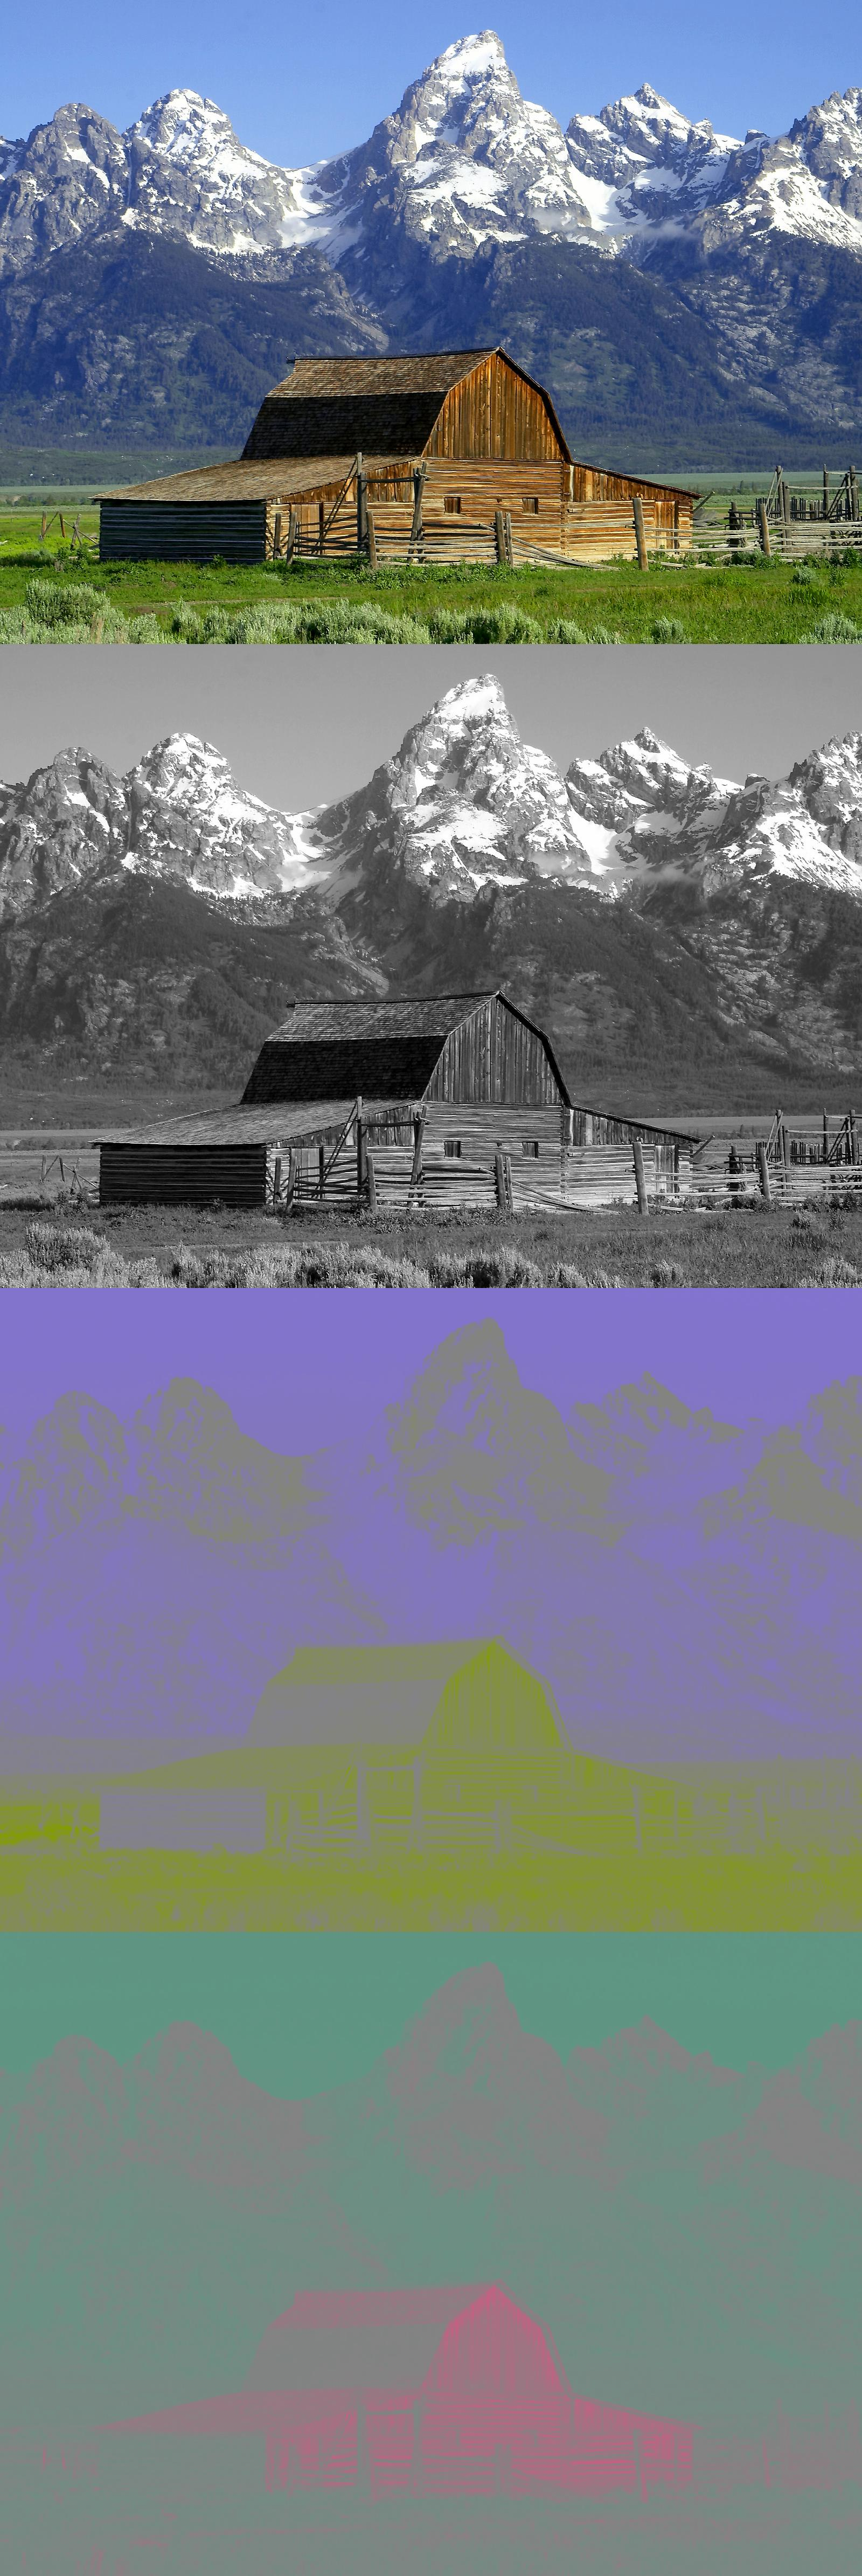
\includegraphics[height=10\baselineskip,keepaspectratio]{figures/Barns_grand_tetons_YCbCr_separation.jpg}
        \caption*{Source: \href{https://commons.wikimedia.org/wiki/File:Barns_grand_tetons_YCbCr_separation.jpg}{Mike1024}, Public domain, via Wikimedia Commons}
      \end{figure}
    \end{column}
  \end{columns}
\end{frame}
\begin{frame}{YCbCr: BT.601-7}
  \begin{itemize}
    \item Last updated in 2011 \autocite{BT601}
    \item Targets standard definition transmissions ($\leq$480p)
    \item Designed for compatibility with legacy receivers
    \item Targets the \emph{D65} white point
  \end{itemize}

  \uncover<+->{
    \begin{align}
      Y' & = 0.299R' + 0.587G' + 0.114B'                                             \\
      Cb & = \frac{0.701}{1.402}R' + \frac{-0.587}{1.402}G' + \frac{-0.114}{1.402}B' \\
      Cr & = \frac{-0.299}{1.772}R' + \frac{-0.587}{1.772}G' + \frac{0.886}{1.772}B'
    \end{align}
  }
\end{frame}
\begin{frame}{YCbCr: BT.709-6 version}
  \begin{itemize}
    \item Last updated in 2015 \autocite{BT709}
    \item Revised version targeting HD and HDR transmissions
    \item Drops legacy compatibility in exchange for accurate eye luminance response
    \item Targets the \emph{D65} white point
  \end{itemize}

  \uncover<+->{
    \begin{align}
      Y' & = 0.2126R' + 0.7152G' + 0.0722B'                                                \\
      Cb & = \frac{-0.2126}{1.8556}R' + \frac{-0.7152}{1.8556}G' + \frac{0.9278}{1.8556}B' \\
      Cr & = \frac{0.7874}{1.5748}R' + \frac{-0.7152}{1.5748}G' + \frac{-0.0722}{1.5748}B'
    \end{align}
  }
\end{frame}
\begin{frame}{YCbCr: range}
  \begin{itemize}
    \item Intended for use in analog circuitry
          \begin{itemize}
            \item e.g. 8-bit unsigned integer: $Y' \in [16, 235]$; $Cb, Cr \in [16, 240]$
            \item the extra room is to allow for the carrier signal to under/overshoot
          \end{itemize}
    \item Both matrices as well as the ICC standard expect data in floating point
    \item \emoji{woman-raising-hand}: what is the range?
    \item \emoji{woman-mage}: only BT.601 explains it (\S2.5.2)
    \item $Y' \in [0, 1]$; $Cb, Cr \in [-0.5, 0.5]$
  \end{itemize}
\end{frame}
\begin{frame}{YCbCr: gamma correction}
  \begin{itemize}
    \item YCbCr takes/returns a gamma-corrected RGB signal
          \begin{itemize}
            \item the $'$ in $R'$ earlier denotes that correction
          \end{itemize}
    \item Formally called \emph{opto-electronic transfer function} (OETF)
    \item Accounts for the non-linearity on the image sensor/display device
    \item BT.601 and BT.709 specify the same relationship between luminance $L$ and electrical signal $E$: \begin{equation}
            E = \begin{cases}
              (1.099L^{0.045} - 0.099) & 0.018 < L \leq 1.00 \\
              4.500L                   & 0 \leq L \leq 0.018
            \end{cases}
          \end{equation}
  \end{itemize}
\end{frame}
\begin{frame}{CRT-style gamma correction}
  \begin{itemize}
    \item There is little info on YCbCr's actual usage so let's consider an alternative
    \item Old-school CRT television sets follow a \emph{power law}
    \item The relationship between emitted light $L$ and driving voltage $V$:
          \begin{equation}
            L = V^{\gamma}
          \end{equation}
    \item $\gamma$ depends on the device
    \item The official recommendation, ITU-R BT.1886 \parencite*{BT1886} defaults to $\gamma = 2.4$
  \end{itemize}
\end{frame}
\section{Conclusions}
\begin{frame}{Remarks}
  \begin{itemize}
    \item Colour management is a complex beast
    \item A \emph{seriously} complex beast!
    \item We covered:
          \begin{itemize}
            \item A primer on colour management
            \item The uniqueness of the YCbCr colour space
            \item How to turn a spec into a profile
          \end{itemize}
  \end{itemize}
\end{frame}
\begin{frame}{Remarks}
  \begin{itemize}
    \item We did not cover the actual implementation
    \item That would make for another hour of talk!
    \item The full, annotated profile generation code is available on GitHub
          \begin{itemize}
            \item \faGithub~\href{https://github.com/amyspark/ycbcr-icc-profiles}{amyspark/ycbcr-icc-profiles}
          \end{itemize}
    \item Extra references at the end of this talk's slides
  \end{itemize}
\end{frame}
\begin{frame}{Thank you for watching!}
  \begin{center}
    {
      \large
      \textbf{Got any questions or comments?}
    }
    \begin{itemize}[<*>]
      \item Q+A next
      \item Email: \href{mailto:amy@amyspark.me?subject="FireShonks 2023"}{amy@amyspark.me}
      \item Matrix: \href{https://matrix.to/\#/@amyspark:fairydust.space}{@amyspark:fairydust.space}
    \end{itemize}
  \end{center}
\end{frame}
\end{document}
